\documentclass[12pt]{article}

\usepackage[utf8]{inputenc}
\usepackage[T1]{fontenc}
\usepackage{geometry}
\usepackage{graphicx} %figures
\usepackage{subfig} %subfigures
\usepackage{gensymb} %degree sign
\usepackage{amsmath} %math stuff
\usepackage{bm} %bold stuff
\usepackage[]{algorithm2e} %algorithms
\geometry{a4paper}

\title{Part 17: Linear Basis Functions}

\begin{document}
\date{March 29, 2021}
\maketitle

This should be a fun easy little jaunt into the world of linear basis functions, which will be based heavily on Martin Krasser's post regarding the same subject.

\section{Linear Basis Function Concept}

The idea starts with the basic assumption of any statistical model, with the \textbf{model structure}:

\begin{equation}
f(x)=w^Tx
\end{equation}

\vspace{5mm}

With the \textbf{statistical structure}:

\begin{equation}
y=f(x)+\epsilon
\end{equation}

\vspace{5mm}

Which can be combined into a \textbf{statistical model structure}:

\begin{align*}
Y \sim N(f(x),\beta^{-1})
\end{align*}

\vspace{5mm}

Where we are assuming the model $f(x)$ is distributed normally with a mean (given by the model structure) and variance $\beta^{-1}$ for inputs $x$ and outputs $y$. Like all distributions this has a likelihood $L(x)=\Pi_i^N N(f(x_i),\beta^{-1})$ and like all normal distributions has an analytical likelihood (that we will not discuss because we've gone over it before).

\section{Making it Bayesian}

How can we make this Bayesian? Of course we need a prior. The prior we will use is:

\begin{align*}
w \sim N(0,\alpha^{-1} I)
\end{align*}

\vspace{5mm}

Which will constrain $w$ in the hyperparameter optimization around 0 with some variance $\alpha^{-1}$. The MLE estimate for the hyperparameters $w$ (or rather MAP estimate because it has a prior) is as follows:

\begin{align*}
\hat{w}=\beta (\alpha+\beta \Phi \Phi^T)^{-1} \Phi^T Y
\end{align*}
\begin{align*}
\hat{\Sigma}_{w}= (\alpha+\beta \Phi \Phi^T)^{-1}
\end{align*}

\vspace{5mm}

Which is also normally distributed. Note that $\Phi(x)$ is the design matrix for all inputs $x$, which forms the backbone of the basis function. So if we have a linear basis function we have $\phi(x)=[1,x]$ and for a second order polynomial we have $\phi(x)=[1,x,x^2]$ and so on and so forth. The capital letter $\Phi(x)$ just indicates this matrix calculation for all $x$ in a group.

\section{Regression}

The most important part is of course regression! Using the optimal MLE hyperparameters we get a mean and covariance function (to take the standard deviation at a single point we take the sum of a column of this covariance matrix square rooted):

\begin{equation}
\hat{y}=\hat{w}^T x
\end{equation}
\begin{equation}
\hat{\Sigma}_{y}=\phi(x)^T \hat{\Sigma}_{w} \phi(x) + \beta^{-1}
\end{equation}

\vspace{5mm}

As an example we generate data $X$ and $Y$ for a linear problem with normally distributed errors and get the following:

\begin{figure}[h]
\centering
\subfloat[][]{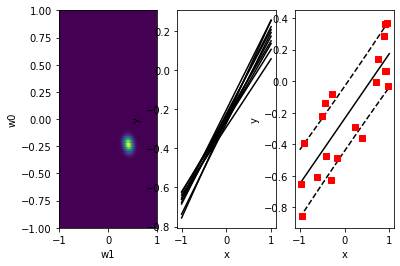
\includegraphics[width=0.4\textwidth]{Post_17_linear}}
\subfloat[][]{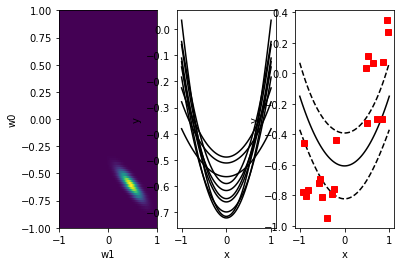
\includegraphics[width=0.4\textwidth]{Post_17_poly}}

\subfloat[][]{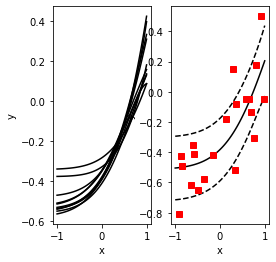
\includegraphics[width=0.4\textwidth]{Post_17_gauss}}
\caption{(a) $[1,x]$ (b) $[1,x^2]$, (c) $[1,K_{SE}(x,\mu=2,\sigma=0.1)]$}
\end{figure}

\end{document}